\documentclass[letter,11pt]{article}

\usepackage[spanish,es-nodecimaldot]{babel}
\usepackage[utf8]{inputenc}

\usepackage{lmodern}
\usepackage[T1]{fontenc}
\usepackage{textcomp}

\usepackage{framed}
\usepackage[svgnames]{xcolor}
\colorlet{shadecolor}{Gainsboro!50}

\usepackage{graphicx}
\usepackage{pstricks}

\usepackage{anysize}
\marginsize{3cm}{2cm}{2cm}{3cm}

\usepackage{siunitx}
\usepackage{amsmath}
\usepackage{array}

\usepackage{fancyhdr}
\usepackage{lastpage}
\pagestyle{fancy}
\fancyhf{}
\fancyhead[LE,RO]{Física Básica III}
\fancyfoot[CO,CE]{\thepage\ de \pageref{LastPage}}

\special{papersize=215.9mm,279.4mm}

\usepackage[
    pdfauthor={Carlos Eduardo Caballero Burgoa},%
    pdftitle={Física Básica III},%
    pdfsubject={2do Parcial},%
    colorlinks,%
    citecolor=black,%
    filecolor=black,%
    linkcolor=black,%
    urlcolor=black,
    breaklinks]{hyperref}
\usepackage{breakurl}

\newcommand{\blankpage}{
\newpage
\thispagestyle{empty}
\mbox{}
\newpage
}

\renewcommand{\arraystretch}{1.2}

\begin{document}

\begin{center}
    {\Large \bf{Segundo parcial}}
\end{center}

\noindent\fbox{%
    \parbox{\textwidth}{%
        Estudiante: CABALLERO BURGOA, Carlos Eduardo \\
        Carrera: Ingeniería Electromecánica \\
        Correo: cijkb.j@gmail.com
    }%
}

\vspace{0.5cm}

\begin{enumerate}
\item La región entre dos esferas conductoras concéntricas con radio $a$ y $b$
está llena de un material conductor cuya resistividad vale $0.6 [\Omega-m]$.
Calcule la resistencia entre las esferas, para $a = 2[cm]$ y $b = 4[cm]$.

\begin{itemize}
    \item $1.10 [\Omega]$.
    \item $1.15 [\Omega]$.
    \item \textcolor{red}{$ 1.19 [\Omega]$.}
    \item $1.23 [\Omega]$.
\end{itemize}

\textbf{Solución:}

\begin{figure}[!h]
\centering
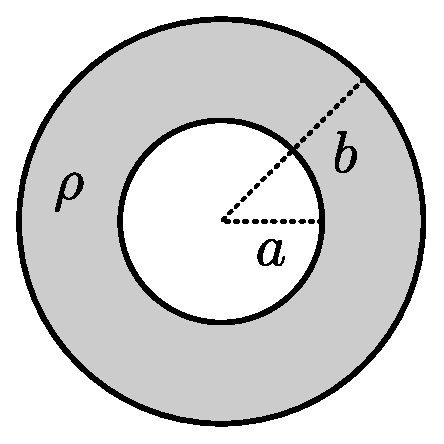
\includegraphics[scale=0.40]{resources/a1.eps}
\end{figure}

La relación entre la resistencia y la resistividad es:

\begin{equation*}
    dR = \rho \frac{dl}{A}
\end{equation*}

Por tanto:

\begin{equation*}
    R = \int_{a}^{b}\rho\frac{dr}{A}
      = \rho\int_{a}^{b}\frac{dr}{4\pi r^2}
      = \frac{\rho}{4\pi}\int_{a}^{b}\frac{dr}{r^2}
      = \frac{\rho}{4\pi}\left(-\frac{1}{r}\Biggr|_{a}^{b}\right)
      = \frac{\rho}{4\pi}\left(\frac{1}{r}\Biggr|_{b}^{a}\right)
      = \frac{\rho}{4\pi}\left(\frac{1}{a}-\frac{1}{b}\right)
\end{equation*}
\begin{equation*}
    R = \frac{0.6}{4\pi}\left(\frac{1}{0.02}-\frac{1}{0.04}\right)
      = 1.1937 [\Omega]
\end{equation*}

\item Un cilindro de $1.5 [m]$ de largo y $1.1 [cm]$ de radio está hecho de una
complicada mezcla de materiales. Su resistividad depende de la distancia ``x''
desde el extremo izquierdo, y cumple con la formula $\rho = a + bx^2$, donde
$a$ y $b$ son constantes. En el extremo de la izquierda, la resistividad es de
$\num{2.25e-8} [\Omega-m]$, en tanto que en el extremo derecho es de
$\num{8.5e-8} [\Omega-m]$. ¿Cuál es la resistencia de esa varilla?

\begin{itemize}
    \item \textcolor{red}{$171 [\mu\Omega]$.}
    \item $168 [\mu\Omega]$.
    \item $160 [\mu\Omega]$.
    \item $151 [\mu\Omega]$.
\end{itemize}

\textbf{Solución:}

\begin{figure}[!h]
\centering
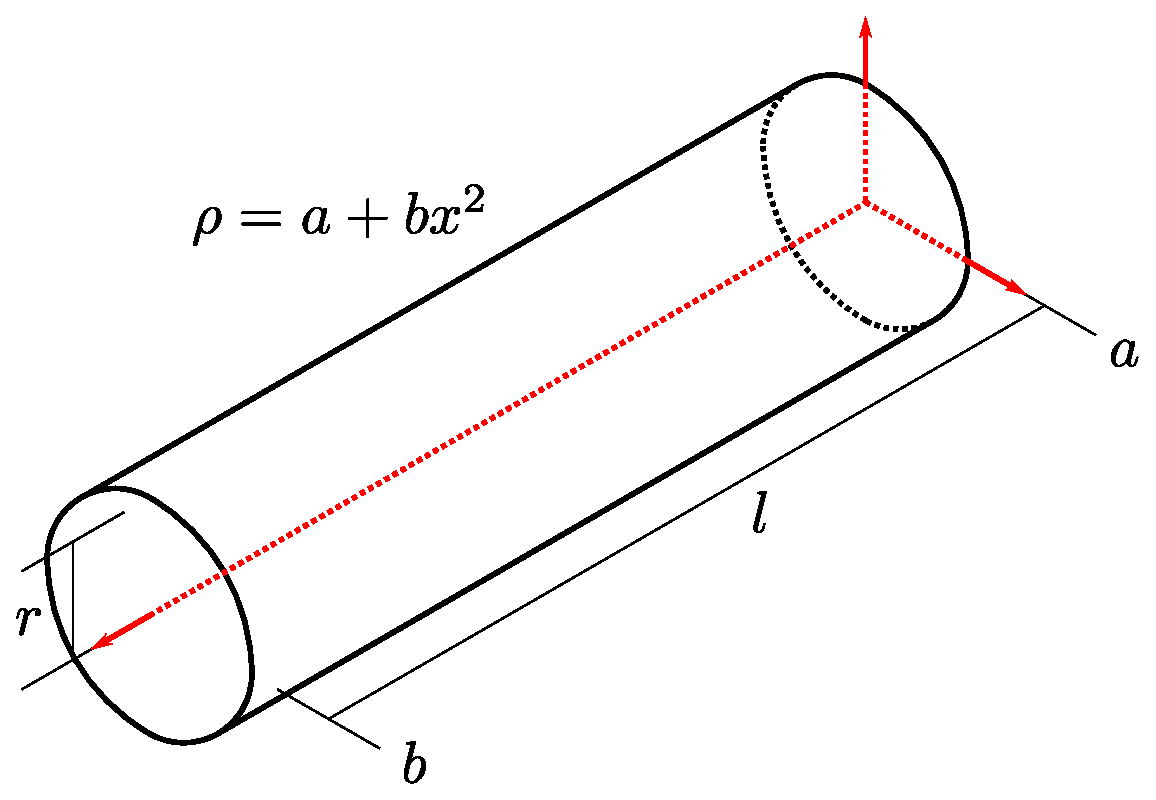
\includegraphics[scale=0.40]{resources/a2.eps}
\end{figure}

Sabiendo los valores de resistividad en los extremos del cilindro, se calculan
los valores de $a$ y $b$:

\begin{equation*}
    \rho(0) = a+b(0)^2 = \num{2.25e-8}
\end{equation*}
\begin{equation*}
    a = \num{2.25e-8}
\end{equation*}
\begin{equation*}
    \rho(1.5) = \num{2.25e-8}+b(1.5)^2 = \num{8.5e-8}
\end{equation*}
\begin{equation*}
    b = \frac{\num{8.5e-8}-\num{2.25e-8}}{(1.5)^2} = \num{2.78e-8}
\end{equation*}

La relación entre la resistencia y la resistividad es:

\begin{equation*}
    dR = \rho\frac{dl}{A}
\end{equation*}

Por tanto:

\begin{equation*}
    R = \int_{0}^{1.5}\rho\frac{dx}{A}
      = \int_{0}^{1.5}\frac{1}{A}(a+bx^2)dx
      = \frac{1}{A}\left(\int_{0}^{1.5}a dx+\int_{0}^{1.5}bx^2 dx\right)
\end{equation*}
\begin{equation*}
    R = \frac{1}{A}\left(ax\Biggr|_{0}^{1.5}
        +b\frac{x^3}{3}\Biggr|_{0}^{1.5}\right)
      = \frac{1}{\pi r^2}\left(a(1.5)+b\frac{(1.5)^3}{3}\right)
      = \num{1.7099e-4}
\end{equation*}
\begin{equation*}
    R = 170.99 [\mu \Omega]
\end{equation*}

\item En el circuito mostrado el resistor de $6 [\Omega]$ consume energía a
razón de $24 [W]$ cuando la corriente a traves de el fluye como se muestra.
Calcule la potencia que disipa el resistor de $19 [\Omega]$.

\begin{figure}[!h]
\centering
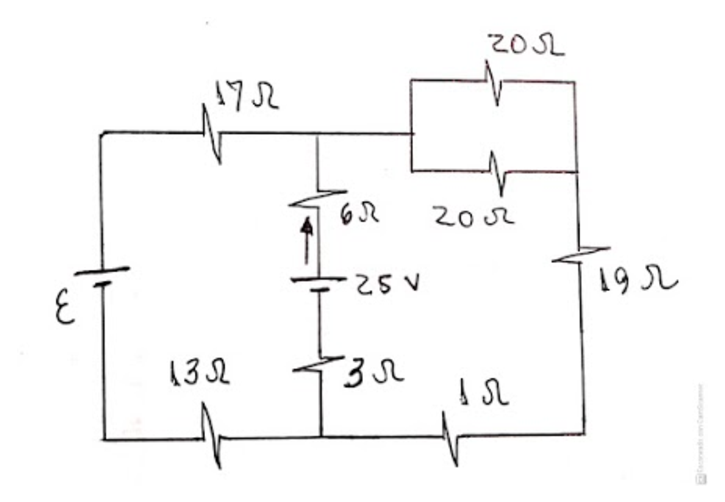
\includegraphics[scale=0.70]{resources/q3.eps}
\end{figure}

\begin{itemize}
    \item $1.03 [W]$.
    \item $1.36 [W]$.
    \item $1.51 [W]$.
    \item $1.63 [W]$.
\end{itemize}

\textbf{Solución:}

\begin{figure}[!h]
\centering
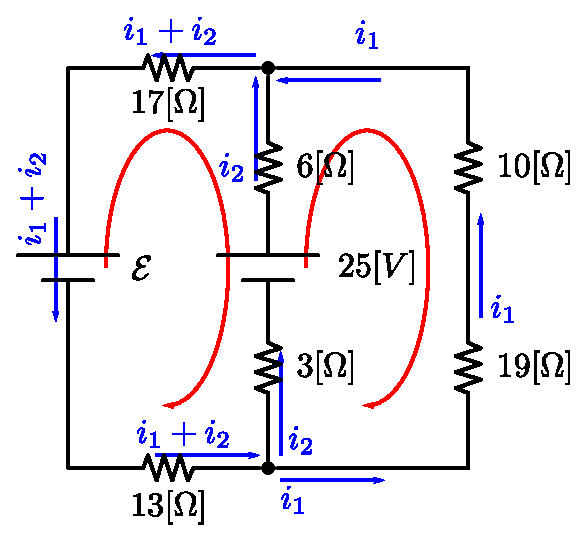
\includegraphics[scale=0.70]{resources/a3.eps}
\end{figure}

Aplicando las reglas de \emph{Kirchhoff}:

\begin{equation*}
    \mathcal{E}+17(i_1+i_2)+6i_2-25+3i_2+13(i_1+i_2)=0
\end{equation*}
\begin{equation*}
    \mathcal{E}+30i_1+39i_2=25
\end{equation*}
\begin{equation*}
    10i_1+19r_1-3i_2+25-6i_2=0
\end{equation*}
\begin{equation*}
    29i_1-9i_2=-25
\end{equation*}

Considerando la potencia que disipa la resistencia de $6 [\Omega]$:

\begin{equation*}
    24 = i_2^2 (6)
\end{equation*}
\begin{equation*}
    \pm 2 = i_2
\end{equation*}

Por tanto $i_1$ es:

\begin{equation*}
    i_1 = \frac{9(\pm 2)-25}{29}
\end{equation*}
\begin{equation*}
    \begin{cases}
        i_1 = -0.2414; (+2) \\
        i_1 = -1.4827; (-2)
    \end{cases}
\end{equation*}

La potencia disipada por la resistencia de $19 [\Omega]$ es:

\begin{equation*}
    P = i_1^2 (19) = 1.1070 [W]
\end{equation*}

\item En el anterior problema calcule la potencia que disipa el resistor de
$17 [\Omega]$.

\begin{itemize}
    \item $50 [W]$.
    \item $51 [W]$.
    \item $52 [W]$.
    \item \textcolor{red}{$53 [W]$.}
\end{itemize}

\textbf{Solución:}

La potencia disipada por la resistencia de $17 [\Omega]$ es:

\begin{equation*}
    P = (i_1+i_2)^2 (17) = 52.5754 [W]
\end{equation*}

\item En el circuito mostrado, calcule el voltaje en el resistor de
$30 [\Omega]$.

\begin{figure}[!h]
\centering
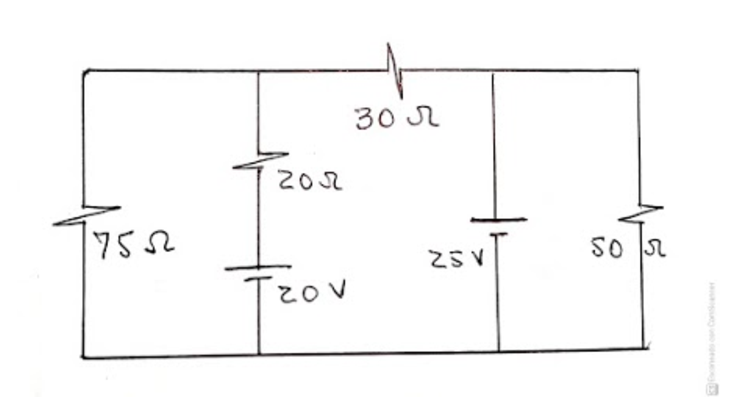
\includegraphics[scale=0.70]{resources/q5.eps}
\end{figure}

\begin{itemize}
    \item \textcolor{red}{$6 [V]$.}
    \item $5.5 [V]$.
    \item $5 [V]$.
    \item $4.5 [V]$.
\end{itemize}

\textbf{Solución:}

\begin{figure}[!h]
\centering
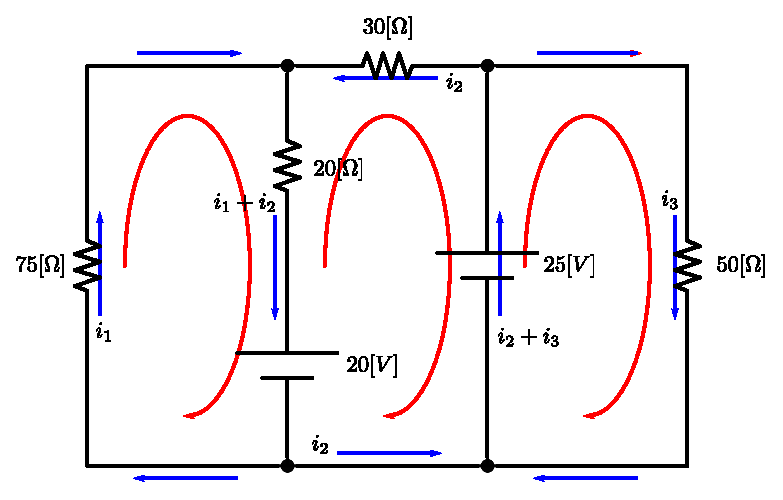
\includegraphics[scale=1.00]{resources/a5.eps}
\end{figure}

Aplicando las reglas de \emph{Kirchhoff}:

\begin{equation*}
    -75i_1-20(i_1+i_2)-20=0
\end{equation*}
\begin{equation*}
    -95i_1-20i_2=20
\end{equation*}
\begin{equation*}
    30i_2-25+20+20(i_1+i_2)=0
\end{equation*}
\begin{equation*}
    20i_1+50i_2=5
\end{equation*}
\begin{equation*}
    50i_3 = -25
\end{equation*}
\begin{equation*}
    i_3 = -0.5
\end{equation*}
\begin{equation*}
    \begin{cases}
        i_1 = -0.2529 \\
        i_2 = 0.20115
    \end{cases}
\end{equation*}

La diferencia de potencial en la resistencia de $30 [\Omega]$ es:

\begin{equation*}
    V = i_2 (30) = 6.0345 [V]
\end{equation*}

\item En el anterior problema, calcule la diferencia de potencial en el resistor
de $75 [\Omega]$.

\begin{itemize}
    \item $16 [V]$.
    \item $17 [V]$.
    \item $18 [V]$.
    \item \textcolor{red}{$19 [V]$.}
\end{itemize}

\textbf{Solución:}

La diferencia de potencial en la resistencia de $75 [\Omega]$ es:

\begin{equation*}
    V = i_1 (75) = -18.97 [V]
\end{equation*}

\item Están conectados en serie una fuente de $\mathcal{E} = 120 [V]$, un
resistor $R = 80 [\Omega]$ y un capacitor con $C = 4 [\mu F]$. A medida que el
capacitor se carga, cuando la corriente en el resistor es de $0.9 [A]$. ¿Cuál es
la carga del capacitor?

\begin{itemize}
    \item $185 [\mu C]$.
    \item \textcolor{red}{$192 [\mu C]$.}
    \item $198 [\mu C]$.
    \item $206 [\mu C]$.
\end{itemize}

\textbf{Solución:}

Considerando la funcion de corriente en funcion del tiempo de carga del
capacitor:

\begin{equation*}
    i = \frac{\mathcal{E}}{R} e^{-t/RC}
      = \frac{120}{80} e^{-t/RC}
\end{equation*}
\begin{equation*}
    e^{-t/RC}=0.6
\end{equation*}
\begin{equation*}
    t = -RC\,ln(0.6)
\end{equation*}

Por tanto, la carga en ese tiempo es:

\begin{equation*}
    q = C_o\mathcal{E} (1-e^{-t/RC})
\end{equation*}
\begin{equation*}
    q = (4\mu)(120) (1-e^{-RC\,ln(0.6)/RC})
\end{equation*}
\begin{equation*}
    q = (4\mu)(120) (1-0.6) = \num{1.92e-4} [C]
\end{equation*}

\item Un capacitor de $6 [\mu F]$, inicialmente descargado, se conecta en serie
con un resistor de $5 [\Omega]$ y una fuente de $\mathcal{E} = 50 [V]$ y
resistencia interna despreciable. En el instante en que el resistor está
disipando energía eléctrica a una tasa de $300 [W]$. ¿Cuánta energia se ha
almacenado en el capacitor?

\begin{itemize}
    \item $650 [\mu J]$.
    \item $643 [\mu J]$.
    \item $635 [\mu J]$.
    \item $630 [\mu J]$.
\end{itemize}

\textbf{Solución:}

La corriente electrica en el momento que la potencia es $300 [W]$ es:

\begin{equation*}
    P = I^2\,R
\end{equation*}
\begin{equation*}
    I = \sqrt{\frac{P}{R}}
\end{equation*}

El tiempo para alcanzar esa corriente electrica en el capacitor es:

\begin{equation*}
    i = \frac{\mathcal{E}}{R}\,e^{-t/RC}
\end{equation*}
\begin{equation*}
    e^{-t/RC} = \frac{R}{\mathcal{E}}i
\end{equation*}
\begin{equation*}
    t = -RC\,ln\left(i\frac{R}{\mathcal{E}}\right)
      = -RC\,ln\left(\frac{R}{\mathcal{E}}\sqrt{\frac{P}{R}}\right)
\end{equation*}

La carga electrica del capacitor en ese tiempo es:

\begin{equation*}
    q = C_o\mathcal{E}\,(1-e^{-t/RC})
\end{equation*}
\begin{equation*}
    q = C_o\mathcal{E}\,\left(1-\left(
        \frac{R}{\mathcal{E}}\sqrt{\frac{P}{R}}\right)\right)
      = \num{6.7621e-5} [C]
\end{equation*}

Por tanto, la energia en el capacitor es:

\begin{equation*}
    U = \frac{q^2}{2C} = \num{3.8105e-4} [J]
\end{equation*}

\item Una espira circular de plastico con radio $R = 0.1 [m]$ y carga positiva
$Q = 1 [\mu C]$, distribuida uniformemente alrededor de la circunferencia de la
espira. Despues esta se hace girar alrededor de su eje central, perpendicular al
plano de la espira, con una frecuencia de $600 [rpm]$. Si la espira esta en una
region donde existe un campo magnetico uniforme de $B = 1 [mT]$ dirigido en
forma paralela al plano de la espira. Calcule la magnitud de la torca magnetica
sobre la espira.

\begin{itemize}
    \item $310 [pN-m]$.
    \item $314 [pN-m]$.
    \item $318 [pN-m]$.
    \item $321 [pN-m]$.
\end{itemize}

\textbf{Solución:}

\item Una barra uniforme tiene una masa de $0.012 [kg]$ y $30 [cm]$ de largo.
Gira sin friccion alrededor de un eje perpendicular a la barra en el punto
``a''. La barra se encuentra en un campo magnetico uniforme que se dirige hacia
la pagina y tiene una magnitud de $B = 0.15 [T]$. Calcular la corriente $I$ en
la barra para que este en equilibrio rotacional cuando esta a un angulo de
$30^\circ$ arriba de la horizontal.

\begin{figure}[!h]
\centering
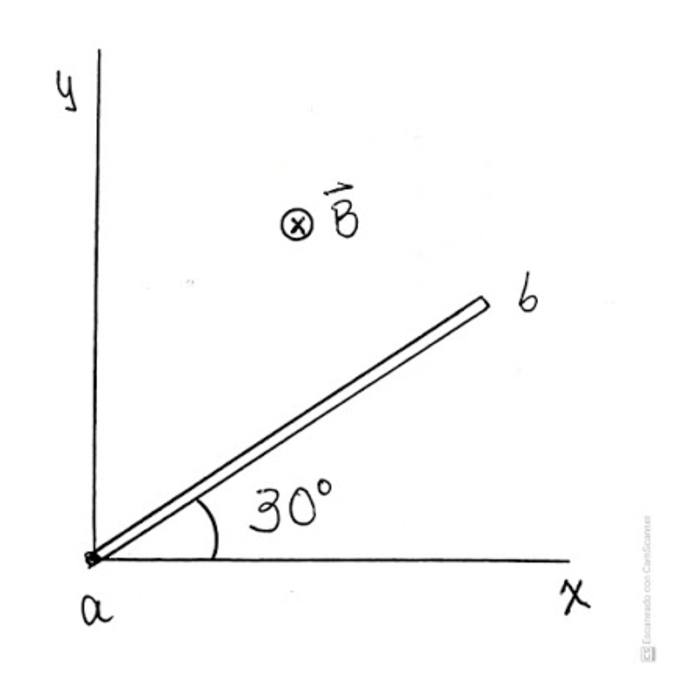
\includegraphics[scale=0.70]{resources/q10.eps}
\end{figure}

\begin{itemize}
    \item $1.63 [A]$.
    \item $1.75 [A]$.
    \item $2.26 [A]$.
    \item $2.61 [A]$.
\end{itemize}

\textbf{Solución:}

\end{enumerate}

\end{document}

